\section{Competitive Ratio General $k$}
\label{app:general_k_proof}
\begin{theorem}
The competitive ratio of Virtual Plus for the case $k \geq 2$ where $t = \alpha n$ can asymptotically be lower bounded by 
\begin{equation}
    C_k >  \max_{\alpha \in [0,1]}  {\alpha}^k \left(\sum_{m = 0}^{k - 1} a_m \ln^m (\alpha)\right) - \alpha a_0
    \hspace{0.15cm }where  \hspace{0.15cm }
    a_m = \left(\frac{\frac{k^k}{(k-1)^{k-m}} - k^m}{m!}\right)(-1)^{m+1}
    \, .
\end{equation}

\end{theorem}
\begin{figure}[ht]
    \centering
    %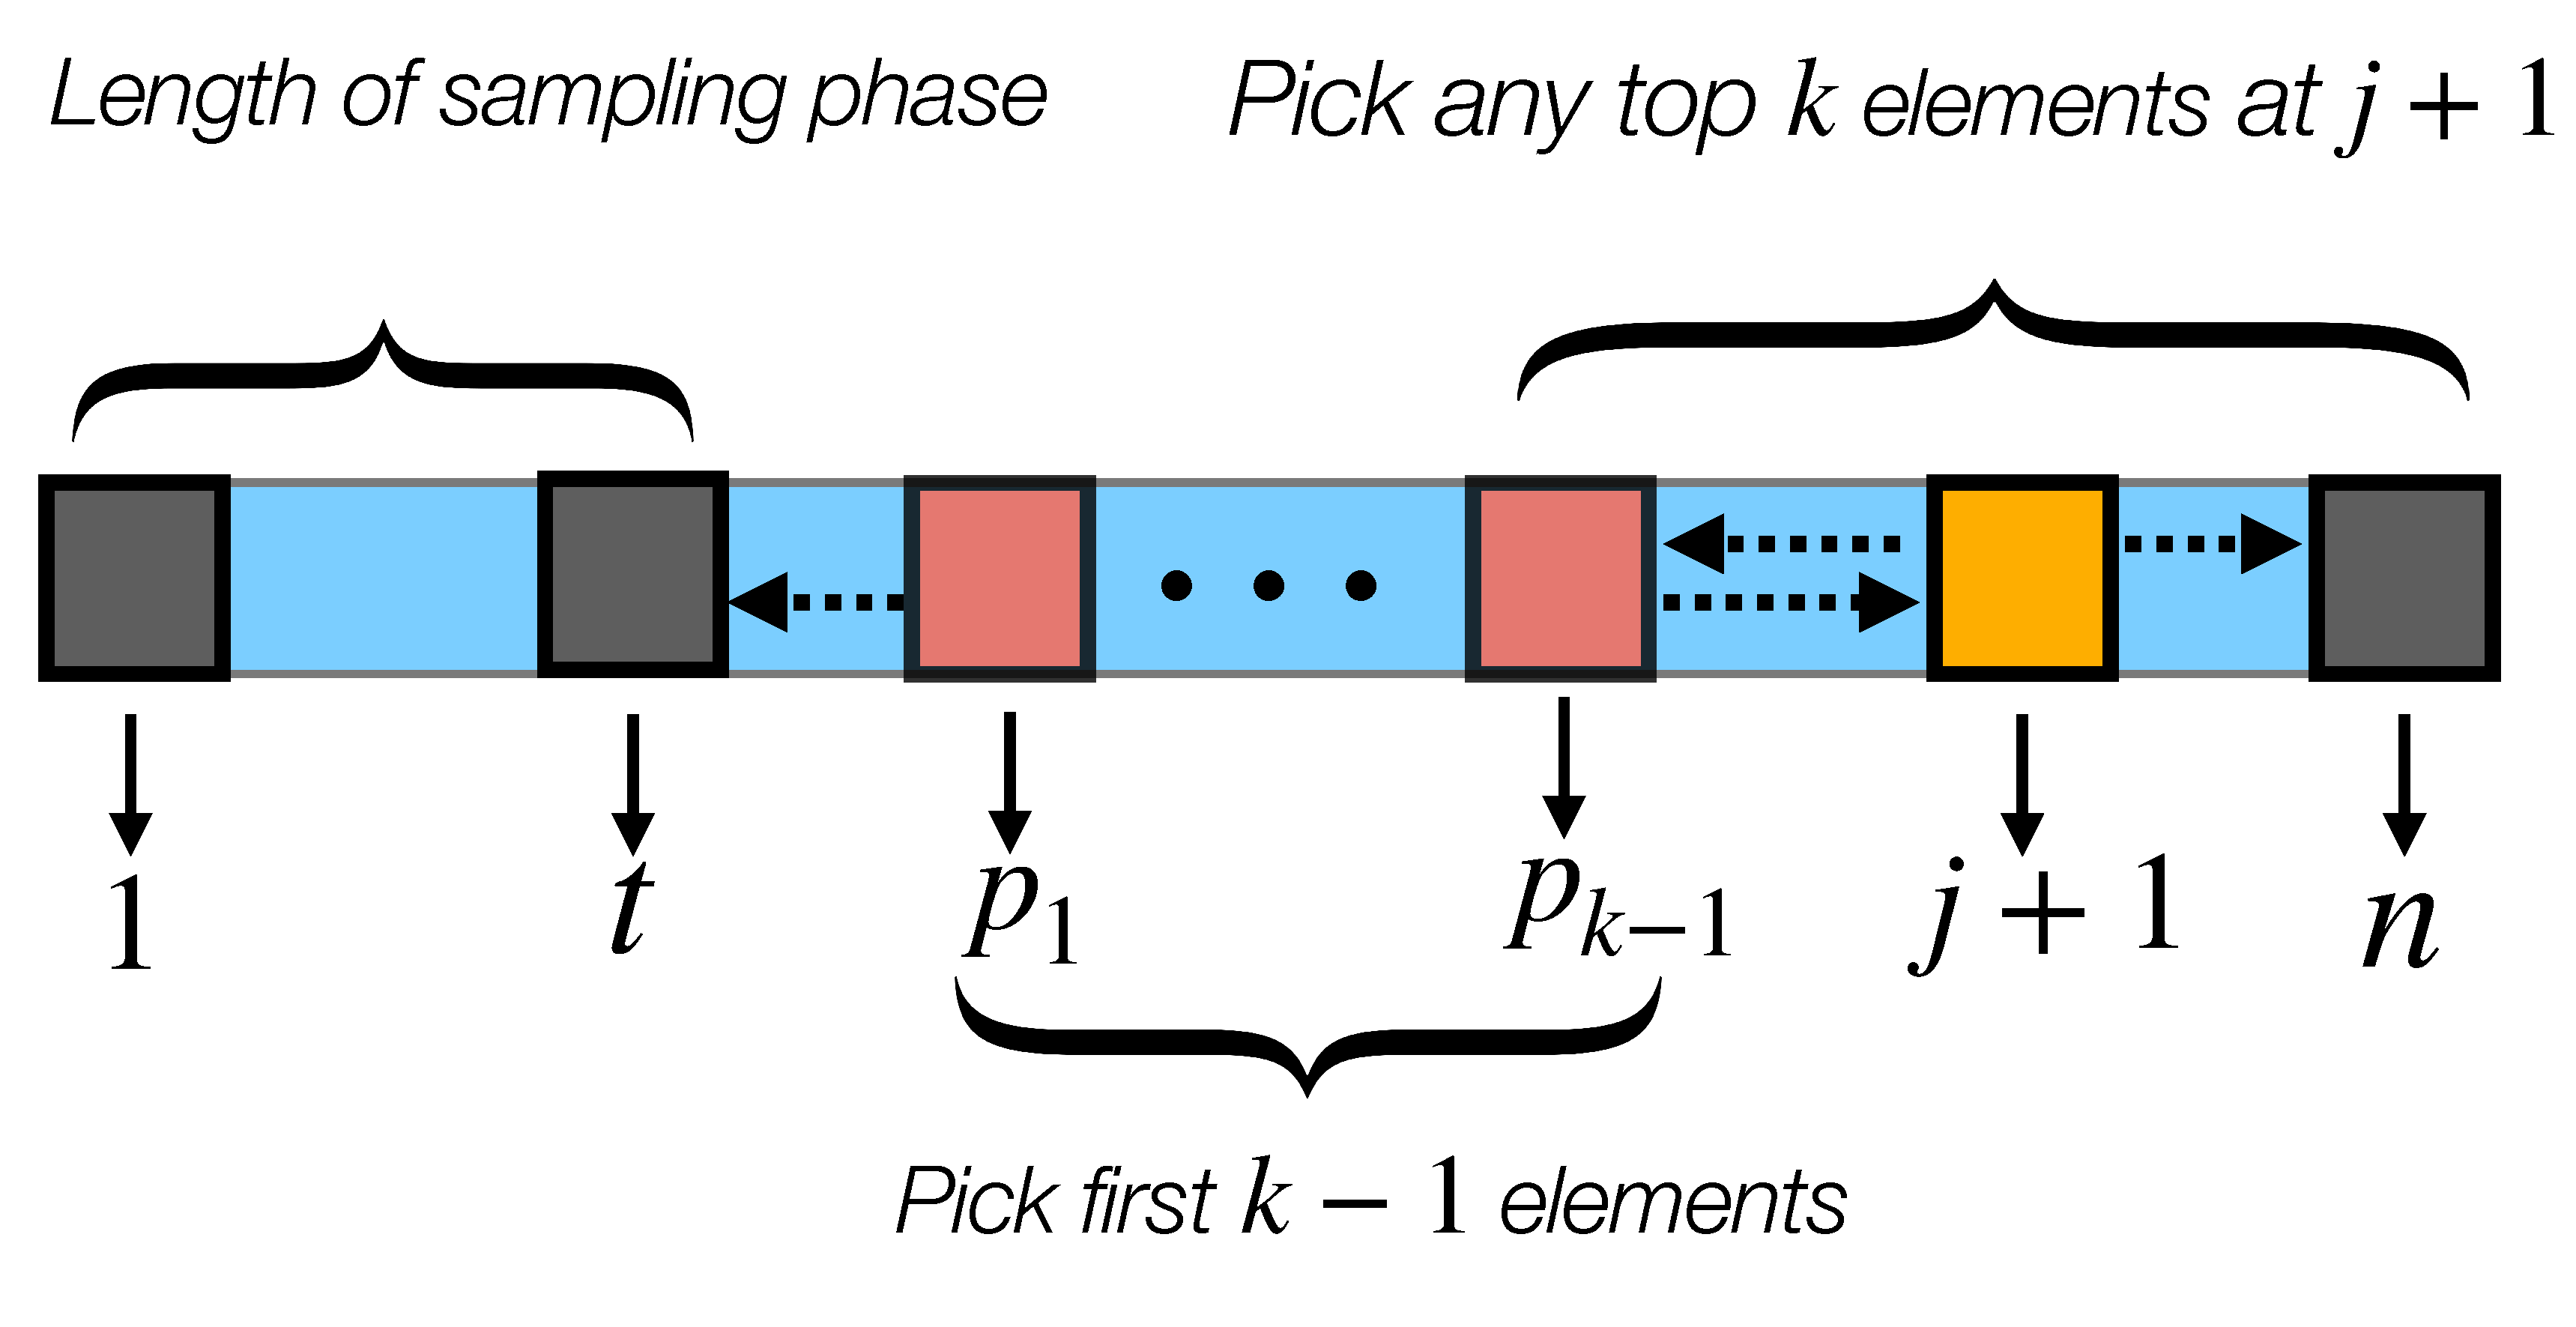
\includegraphics[width=0.50\linewidth]{Figures/virtual_plus_general_k.pdf}
    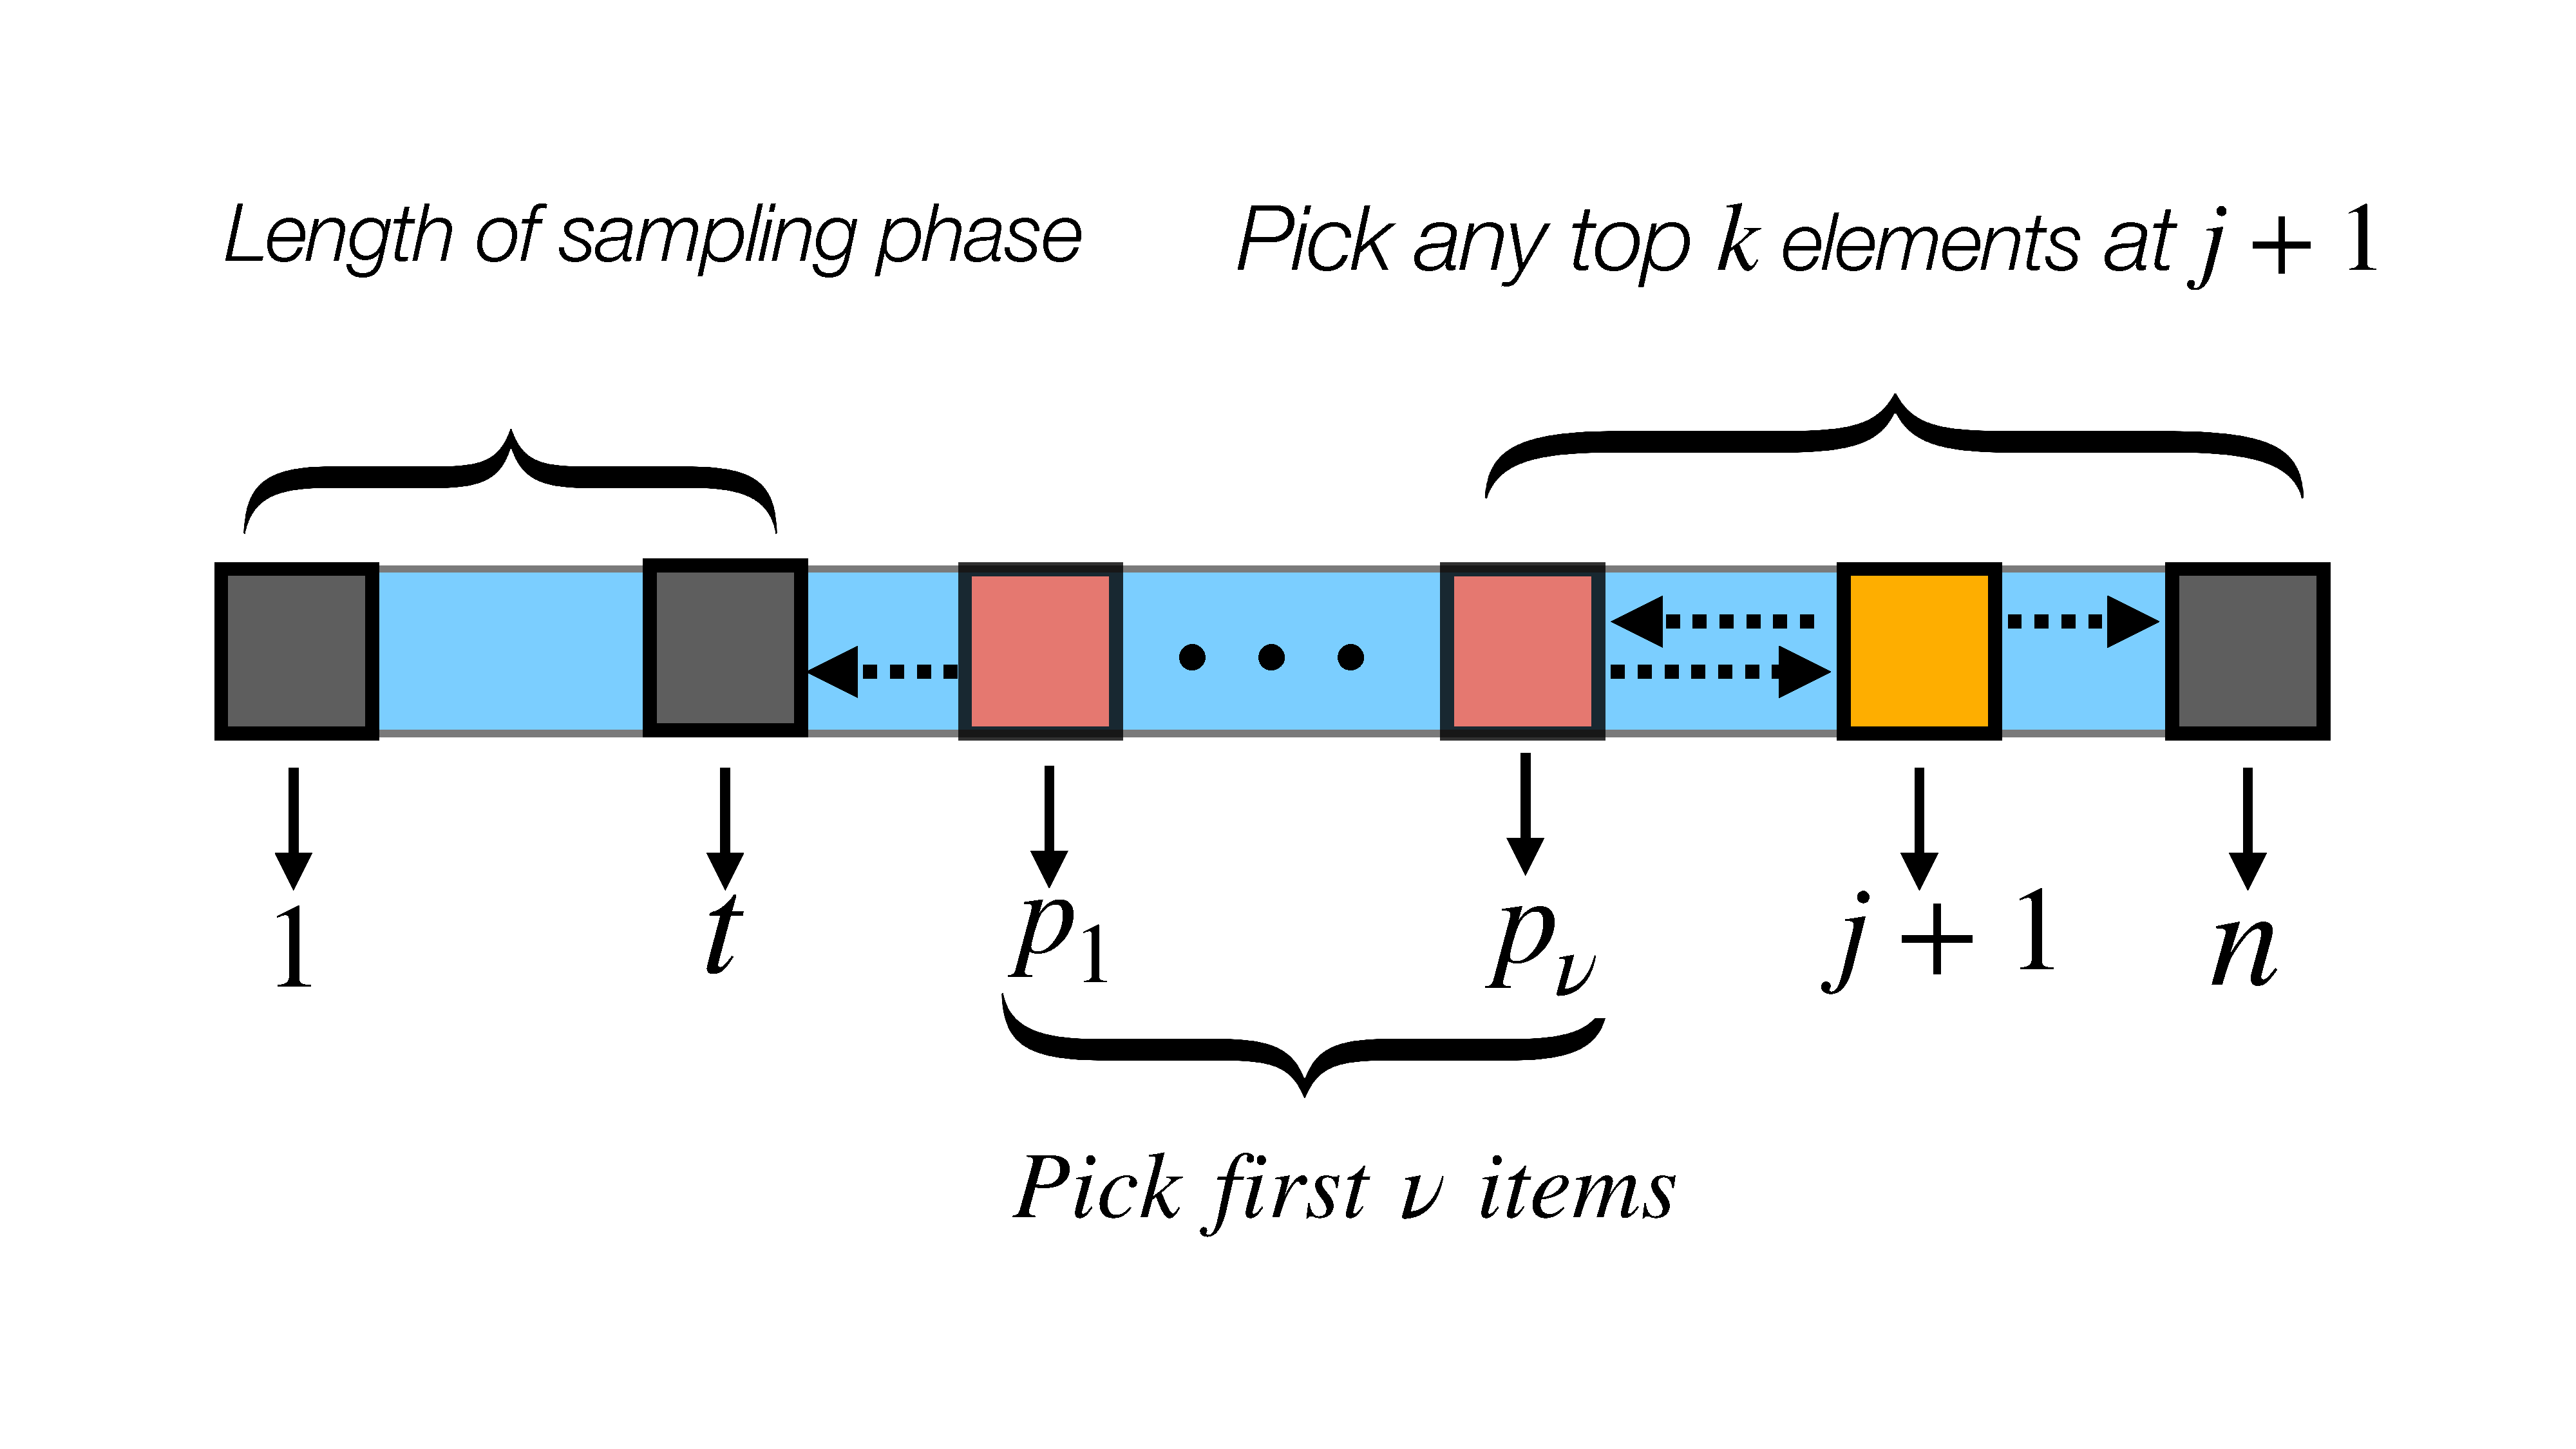
\includegraphics[width=0.50\linewidth]{Figures/general_k.pdf}
    %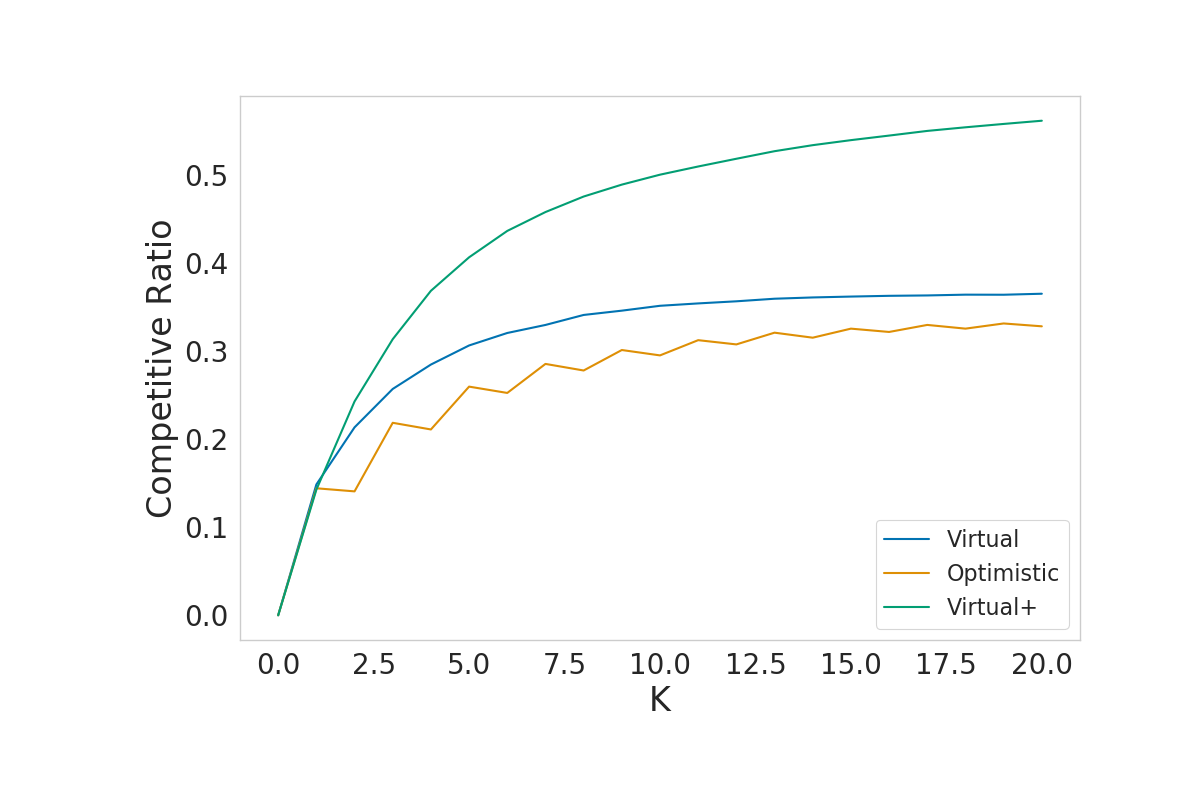
\includegraphics[width=\linewidth]{Figures/Competitive_RatioVar5.png}
    \caption{Virtual+ $k \geq 2$ proof.}
    \label{fig:general_k}
    %\vspace{-5mm}
\end{figure}
\begin{proof}
First note that we can show that the competitive ratio for the $k$-secretary problem is equal to 
\begin{equation}
    C = \frac{1}{k}\sum_{a=1}^k \mathbb{P}(i_a \in S_\mathcal{A}), \label{eq:C_as_sum_prob1}
\end{equation}
where $i_a$ is the index of the $a^{th}$ secretary picked by the offline solution ---i.e. $i_a$ is a top-$k$ secretary of $\mathcal{D}$. 

\begin{align}
    \mathbb{P}(i_a \in S_\mathcal{A}) 
    &= \sum_{j=t}^{n-1} \mathbb{P}(i_a \in S_\mathcal{A} \text{ at time-step }j+1) \label{p_picked_equal_not_filled} \\
    &= \frac{1}{n}\sum_{j=t}^{n-1} \mathbb{P}(|S_{\mathcal{A}}| < k \text{ at time-step } j + 1) \notag
\end{align}

Now, we compute $\mathbb{P}(|S_{\mathcal{A}}| < k \text{ at time-step } j+1)$ by decomposing this probability into the smaller events aka $\mathbb{P}(|S_{\mathcal{A}}| = 1 \text{ at time-step } j+1)$, $\mathbb{P}(|S_{\mathcal{A}}| = 2 \text{ at time-step } j+1)\dots \mathbb{P}(|S_{\mathcal{A}}| = k - 1 \text{ at time-step } j+1)$

We compute the probability of $\mathbb{P}(|S_{\mathcal{A}}| = \nu \text{ at time-step } j+1)$ in the following manner. First of let's say that $\nu$ elements are being selected by the algorithm at the time steps $p_1$, $p_2, \dots p_{\nu}$. In order for element to be selected at position $p_\nu$ that element has to be one of the top $k$ elements up to $j+1$. Therefore we have factor $\frac{k}{j}$ in our equation. Now, in order to make sure that none of the elements are picked after the position $p_\nu$ we need to make sure that the rest of top - $k$ up to $j+1$ appeared before $p_\nu$ therefore we have the factor of $\frac{{p_{\nu} - 1 \choose k - 1}}{{j-1 \choose k - 1}}$. Similarly we calculate recursively for each position $p_{\nu-1} \dots p_1$. However, we also need to make sure that none of the elements are picked in the time interval $[t+1 \dots p_1-1]$
aka before $p_1$ and probability for that is  $\frac{{t \choose k}}{{p_1-1 \choose k}}$ - when the top $k$ elements up to $p_1 - 1$ appear in the sampling phase.
Probability of $\mathbb{P}(|S_{\mathcal{A}}| = \nu \text{ at time-step } j+1)$ is :
\begin{align}
    &= \sum_{t+1 \leq p_1 < p_2 < \dots <p_{k-1} \leq j}\frac{k}{j} \frac{{p_{\nu} - 1 \choose k-1}}{{j-1 \choose k-1}}\frac{k}{p_{\nu} - 1}
    \frac{{p_{{\nu}-1} - 1 \choose k-1}}{{p_{\nu} - 2 \choose k-1}}\frac{k}{p_{\nu-1} - 1}\dots \frac{k}{p_2 - 1}\frac{{p_1 - 1 \choose k - 1}}{{p_2 - 2 \choose k-1}} \frac{{t \choose k}}{{p_1-1 \choose k}}\\
    & = \frac{t(t-1)\dots(t-k+1)}{j(j-1)\dots (j - k + 1)}\sum_{t+1 \leq p_1 < p_2 < \dots <p_{k-1} \leq j}
    \frac{k^{\nu}}{(p_\nu-k)(p_{\nu-1} - k)\dots(p_1 - k)}
\end{align}

Therefore, probability of not being overfilled before time step j + 1:
\begin{align}
    & \frac{t(t - 1)...(t - k + 1)}{j (j - 1) \dots (j - k + 1)} \Big(1 + k\hspace{-1em}\sum_{p_1 = t + 1\dots j}^{}\frac{1}{p_1 - k} + \dots
    + {k^{k - 1}}\hspace{-2em}\sum_{\substack{p_1 = t + 1 \dots j \\\vdots\\ p_{k-1} = t + 1 \dots p_{k-2}}}\frac{1}{(p_1 - k)\dots (p_{k-1} - k)} \Big)\\
    & = 
    \frac{t(t - 1)...(t - k + 1)}{j (j - 1) \dots (j - k + 1)} \Big(1 + k\hspace{-0.5 em}\sum_{p_1 = t + 1}^{j}\frac{1}{p_1 - k} + 
     \dots  +
     {k^{k - 1}}\sum_{p_1 = t + 1}^{j}\frac{1}{ (p_{1} - k)} \dots \sum_{p_{k-1} = t + 1}^{p_{k-1}}\frac{1}{ (p_{k-1} - k)} \Big) 
\end{align}

Now we make use of the  
Lemma~\ref{lemma_two}:
\begin{align}
 = 
     \frac{t(t - 1)\dots (t - k + 1)}{j(j - 1)\dots(j - k + 1)}(1 + {k}\frac{1}{1!}\ln (\frac{j - k}{t}) + {k^2}\frac{1}{2!}\ln^2(\frac{j - k}{t}) + \dots + {k^{k - 1}}\frac{1}{(k-1)!}\ln^{k - 1}(\frac{j - k}{t})\Big)
\end{align}

Then we get that the total competitive ratio: 
\begin{align}
     & \frac{1}{n}\sum_{j = t}^{n - 1}
     \frac{t(t - 1)\dots (t - k + 1)}{j(j - 1)\dots(j - k + 1)}(1 + {k}\frac{1}{1!}\ln (\frac{j - k}{t}) + {k ^ 2}\frac{1}{2!}\ln^2(\frac{j - k}{t}) + \dots + {k^{k - 1}}\frac{1}{(k-1)!}\ln^{k - 1}(\frac{j - k}{t})\Big)\\
     & \geq
     \frac{1}{n}\int_{j = t}^{n}
     \frac{t(t - 1)\dots (t - k + 1)}{j(j - 1)\dots(j - k + 1)}\Big(1 + {k}\frac{1}{1!}\ln (\frac{j - k}{t}) + {k^2}\frac{1}{2!}\ln^2(\frac{j - k}{t}) + \dots + {k^{k - 1}}\frac{1}{(k-1)!}\ln^{k - 1}(\frac{j - k}{t})\Big)\\
     & \geq
     \frac{1}{n}\int_{j = t}^{n}
     \frac{t(t - 1)\dots (t - k + 1)}{j^k}\Big(1 + {k}\frac{1}{1!}\ln (\frac{j - k}{t}) + {k^2}\frac{1}{2!}\ln^2(\frac{j - k}{t}) + \dots + {k^{k - 1}}\frac{1}{(k-1)!}\ln^{k - 1}(\frac{j - k}{t})\Big)\\
\end{align}
Now notice that:
\begin{equation}
    \label{identity_two}
    \int\frac{1}{a!} \frac{\ln^a(x)}{x^k} dx = - \frac{1}{x^{k - 1}}\sum_{m = 0}^{a}\frac{1}{m!}(k -1)^{m - 1 -a }\ln^m(x)
\end{equation}
Then we make use of this identity and get that competitive ratio is:
\begin{align}
     & \geq\frac{t(t - 1)\dots (t - k + 1)}{n}
     \Big(\sum_{a = 0}^{k - 1}- \frac{1}{j^{k - 1}}{ k ^ a }\sum_{m = 0}^{a}\frac{1}{m!}(k -1)^{m - 1 -a }\ln^m(\frac{j - k}{t}) \Big) \Big|_{j = t}^{n}\\
     & =
     \frac{t(t - 1)\dots (t - k + 1)}{n}\Big(- \frac{1}{j^{k - 1}}\sum_{m = 0}^{k - 1}\frac{1}{m!}\Big(\sum_{a = m}^{k - 1}{k ^ a}(k - 1)^{m - a - 1}\Big)\ln^m{(\frac{j - k}{t})}\Big)\Big|_{j = t}^{n}
\end{align}
Now as $t = \alpha n $ where $\alpha \in (0,1)$ and as $n \xrightarrow{}\infty$ our competitive rate becomes:
\begin{align}
    & \alpha \Big(\sum_{a = 0}^{k - 1}{ k ^ a }{(k - 1)}^{-1 - a}\Big) - \alpha^k\Big(\sum_{m=0}^{k - 1}\frac{1}{m!}\Big(\sum_{a = m}^{k - 1}{ k ^ a }(k - 1)^{m - a - 1}\Big)\ln^m(\frac{1}{\alpha})\Big)\\
    & = \alpha\left({\left(\frac{k}{k-1}\right)}^{k} - 1\right) - \alpha^k\left(\sum_{m-0}^{k-1}\left(\frac{\frac{k^k}{(k-1)^{k-m}} - k^m}{m!}\right)(-1)^{m+1}\ln^m(\alpha)\right)
\end{align}

\begin{lemma} 
\label{lemma_two}
Let $f_i \,, \,i = 1 \ldots k$ be decreasing positive functions then we have 
\begin{equation}
    \sum_{p_1=a_1}^{b_1} \ldots \sum_{p_k=a_k}^{p_{k-1}} f_1(p_1) \ldots f_k(p_k)
    \geq \int_{x_1=a_1}^{b_1+1} \ldots \int_{x_k = a_k}^{x_{k-1}+1}  f_1(x_1) \ldots f_k(x_k) dx_1\dots dx_k
\end{equation}
\end{lemma}
\begin{proof}
    The proof consists in noticing that since the functions $f_i \,, \,i = 1 \ldots k$ are decreasing and positive we have, 
    \begin{equation}
        f_1(p_1) \ldots f_k(p_k) \geq  f_1(p_1) \ldots  f_{k-1}(p_{k-1})\int_{x_k = p_k}^{p_k+1} f_k(x_k) dx_k
    \end{equation}
    Thus, by summing this inequality for $p_k= a_k \ldots p_{k-1}$, we get
    \begin{equation}
    \sum_{p_k=a_k}^{p_{k-1}} f_1(p_1) \ldots f_k(p_k)
    \geq  f_1(p_1) \ldots  f_{k-1}(p_{k-1})  \int_{x_k = a_k}^{p_{k-1}+1} f_k(x_k) dx_k
    \end{equation}
    Now, because the functions $f_i \,, \,i = 1 \ldots k$ are decreasing and positive we have, 
     \begin{align}
    \sum_{p_k=a_k}^{p_{k-1}} f_1(p_1) \ldots f_k(p_k)
    \geq  f_1(p_1) \ldots  f_{k-2}(p_{k-2})  \int_{x_{k-1} = p_{k-1}}^{p_{k-1}+1} f_{k-1}(x_{k-1})  \int_{x_k = a_k}^{p_{k-1}+1} f_k(x_k) dx_{k-1}dx_k \\
    \geq f_1(p_1) \ldots  f_{k-2}(p_{k-2})  \int_{x_{k-1} = p_{k-1}}^{p_{k-1}+1} f_{k-1}(x_{k-1})  \int_{x_k = a_k}^{x_{k-1}} f_k(x_k) dx_{k-1}dx_k 
    \end{align}
    where for the last inequality we used the fact that $x_{k-1} \in [p_{k-1}, p_{k-1}+1]$.
    Finally, by summing for $p_{k-1} = a_{k-1} \ldots p_{k-2}$, we get,
    \begin{equation}
    \sum_{p_{k-1}=a_{k-1}}^{p_{k-2}}  \sum_{p_k=a_k}^{p_{k-1}} f_1(p_1) \ldots f_k(p_k)
    \geq f_1(p_1) \ldots  f_{k-2}(p_{k-2})  \int_{x_{k-1} = p_{k-1}}^{p_{k-1}+1} f_{k-1}(x_{k-1})  \int_{x_k = a_k}^{x_{k-1}} f_k(x_k) dx_{k-1}dx_k
    \end{equation}
    With a recursive argument, we finally get,
    \begin{equation}
    \sum_{p_1=a_1}^{b_1} \ldots \sum_{p_k=a_k}^{p_{k-1}} f_1(p_1) \ldots f_k(p_k)
    \geq \int_{x_1=a_1}^{b_1+1} \ldots \int_{x_k = a_k}^{x_{k-1}+1}  f_1(x_1) \ldots f_k(x_k) dx_1\dots dx_k
\end{equation}
\end{proof}

\end{proof}

\subsection{Table of $C_k$}

\begin{table}[]
    \centering
    \begin{tabular}{ccccccccccc}
     \toprule
          $k$ & 2 &3 & 4 & 5 & 100 & 200 &300 &400 & 500 & 600\\
         \midrule
        $C_k$ & .4273&.4575&.4769&.4906&.5959&.6062&.6108&.6136&.6156&.6170 \\
        $\alpha_k$ & .3824 &.3867&.3884&.3890&.3781 &.3755 &.3743&.3735&.3729&.3726 \\
        \bottomrule
    \end{tabular}
    \caption{Values of the Competitive ratio $C_k$ and the associated optimal threshold $\alpha_k$ for \algoname. Note that for $5\leq k\leq 100$ the competitive ratio of \textsc{Single-Ref} provided by~\citet{albers2020new} outperforms \algoname's competitive ratio. However, our analysis provides a tractable way for the competitive ratio that scales with $k$ since the computation of the function to optimize (and its gradients) in Theorem~\ref{thm:K_2_theorem1} is a $O(k)$.}
    \label{tab:C_k}
\end{table}